\chapter{正弦波振荡器}

\section{概述}

振荡器是一种无需外加激励信号,自动将直流电源能量转换为一定波形的交变振荡信号能量的转换电路。

振荡器在无线通信中的作用:在发射端负责生成载波 (用于承载有用信息的高频正弦波);在接收端负责生成本振信号 (用于混频)。

振荡器的主要类型:

\begin{equation}
    \notag
    \text{振荡器} \left\{
        \begin{array}{l}
            \text{按输出振荡波形} \left\{
                \begin{array}{l}
                    \text{正弦波振荡器} \\
                    \text{非正弦波振荡器}
                \end{array}
            \right. \\
            \text{按工作原理} \left\{
                \begin{array}{l}
                    \text{反馈式振荡器} \\
                    \text{负阻式振荡器}
                \end{array}
            \right. \\
            \text{按器件} \left\{
                \begin{array}{l}
                    \text{$LC/RC$振荡器} \\
                    \text{石英晶体振荡器} \\
                    \text{陶瓷振荡器}
                \end{array}
            \right.
        \end{array}
    \right.
\end{equation}

\section{振荡的起振、平衡、稳定条件 \textcolor{red}{$\bigstar$}}

凡是从输出信号中取出一部分反馈到输入端作为输入信号,无需外部提供激励信号,能产生等幅正弦波输出,称为正反馈振荡器。

当 $\dot{A} \dot{F} = 1$ 时,振荡进入平衡状态。

起振方式:在电源接通时,电路中存在扰动;LC谐振回路选频;由反馈网络反馈到放大器的输入端,又被进一步地放大;如此反复,输出端不断地得到一个增大的自激振荡,且反馈信号的相位与前一输入信号相同,形成正反馈。从而完成了起振的目的。

振荡的起振条件:振幅条件 $A(\omega_0) F(\omega_0) > 1$;相位条件 $\varphi_A(\omega_0) + \varphi_F(\omega_0) = 2 n \pi$。

振荡的平衡条件:振幅条件 $|A||F| = 1$;相位条件 $\varphi_A + \varphi_F = 2 n \pi$。

振荡的稳定条件:振幅条件 $\dfrac{\partial A}{\partial V_{om}} < 0$;相位条件 $\dfrac{\partial \varphi_{\Sigma}}{\partial \omega} < 0$。

\section{电感耦合型反馈振荡器}

互感耦合振荡器是依靠线圈之间的互感耦合实现正反馈的,耦合线圈同名端的正确位置的放置,选择合适的耦合量M,使之满足振幅起振条件很重要。

互感耦合振荡器有三种形式:调基电路、调集电路、调发电路。

互感耦合振荡器在调整反馈 (改变$M$) 时,基本上不影响振荡频率。但由于分布电容的存在,在频率较高时,难于做出稳定性高的变压器。因此,它们的工作频率不宜过高,一般应用于中、短波波段。

根据 $h$ 参数等效电路分析可知互感耦合振荡器的振荡频率:

\begin{equation}
    f_0 = \frac{1}{2 \pi} \sqrt{\frac{1}{LC}}
\end{equation}

瞬时极性法判断互感耦合$LC$振荡器相位:

(1) 先判断是共基、共射还是共集电路;

(2) 把正确的信号输入端标上“$+$”,把地标上“$-$”;

(3) 通过瞬时电流的流向帮助中间点的极性判断;

(4) 有抽头电路时,先找到接地那一端,抽头处的极性与不接地的那一端极性相同;

(5) 循环一圈后,仍为“$+$”则符合起振相位条件,否则就不可能起振。

\begin{figure}
    \centering
    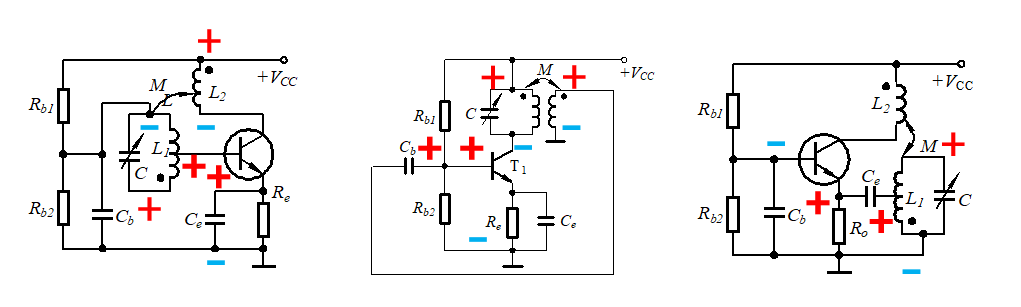
\includegraphics[scale=0.8]{image/Picture6.png}
    \caption{调集、调基、调发电路及瞬时极性判断}
\end{figure}

\section{三端式反馈振荡器 \textcolor{red}{$\bigstar$}}

三端式振荡器的优点:其工作频率约在几MHz到几百MHz的范围,频率稳定度也比互感耦合振荡电路高一些,约为 $10^{-3} \sim 10^{-4}$ 量级,采取一些稳频措施后,还可以再提高一点。

\subsection{电感反馈式三端振荡器}

电感反馈三端振荡器的反馈系数:

\begin{equation}
    F = \frac{L_2 + M}{L_1 + M}
\end{equation}

电感反馈三端振荡器的振荡频率:

\begin{equation}
    f_{\text{osc}} = \frac{1}{2 \pi \sqrt{L_{\Sigma} C}}
    = \frac{1}{2 \pi \sqrt{(L_1 + L_2 + 2M) C}}
\end{equation}

电感反馈三端振荡器的优点:电感间有互感,反馈较强,容易起振;
改变 $C$ 可调节振荡频率,基本不影响反馈系数。

电感反馈三端振荡器的缺点:振荡波形不好,失真大;振荡频率不能太高,因为频率太高,$L$ 太小且分布参数的影响太大。

\subsection{电容反馈式三端振荡器}

电容反馈三端振荡器的反馈系数:

\begin{equation}
    F = \frac{C_1}{C_2}
\end{equation}

电容反馈三端振荡器的振荡频率:

\begin{equation}
    f_{\text{osc}} = \frac{1}{2 \pi \sqrt{L C_{\Sigma}}}
    = \frac{1}{2 \pi \sqrt{L \left(\frac{C_1 C_2}{C_1 + C_2}\right)}}
\end{equation}

电容反馈三端振荡器的优点:振荡波形好;频率稳定度较高;工作频率可以做得较高。

电容反馈三端振荡器的缺点:调 $C_1$ 或 $C_2$ 改变振荡频率时,反馈系数也将改变。

若在 $L$ 两端并上一个可变电容器,并令 $C_1$ 与 $C_2$ 为固定电容,则在调整频率时,基本上不会影响反馈系数。

\subsection{三端振荡器相位平衡条件与判断准则 \textcolor{red}{$\bigstar$}}

\begin{figure}[htbp]
    \centering
    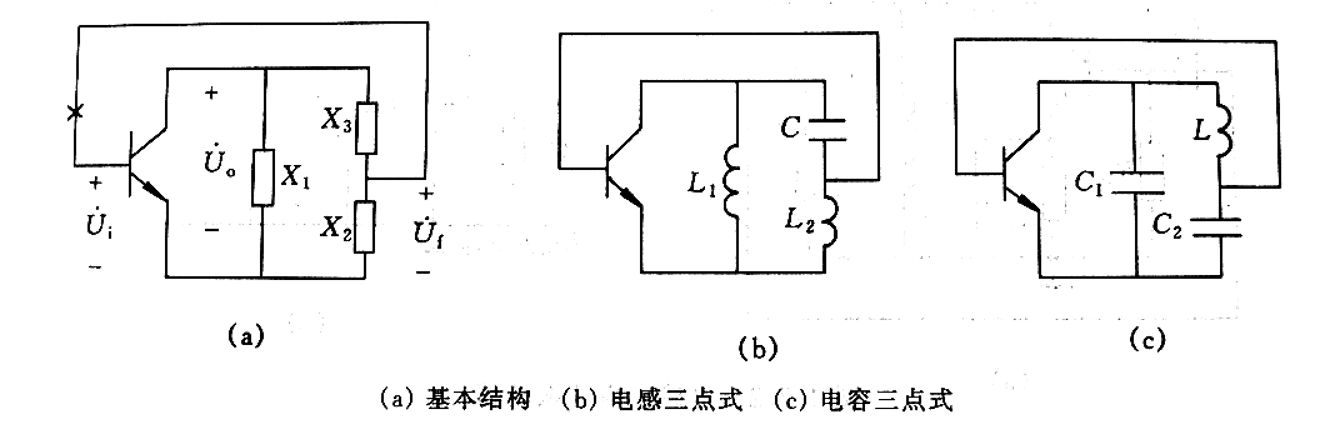
\includegraphics[scale=0.6]{image/Picture7.png}
    \caption{三点式振荡器结构}
\end{figure}

三点式电路组成的相位判据:在三点式电路中,$LC$ 回路中与发射极相连接的两个电抗元件必须为同性质,另外一个电抗元件必须为异性质。

与发射极相连接的两个电抗元件同为电容时的三点式电路,称为电容三点式电路,也称为考毕兹 (Colpitts) 电路。

与发射极相连接的两个电抗元件同为电感时的三点式电路,称为电感三点式电路,也称为哈特莱 (Hartley) 电路。

\section{振荡器的频率稳定性问题}

\subsection{衡量振荡器的指标}

准确度:离中心的偏离程度 (体现“误差”)。

稳定度:变化摆动的剧烈程度 (体现“方差”)。

振荡器的绝对频率准确度、相对频率准确度、频率稳定度分别为:

\begin{equation}
    \Delta f = f - f_0, \quad \frac{\Delta f}{f_0} = \frac{f - f_0}{f_0}, \quad \left. \frac{\Delta f}{f_0} \right|_{\Delta t}
\end{equation}

\subsection{影响频率稳定度的因素}

(1) $LC$ 器件的稳定度:选择稳定度好的$LC$器件、温度补偿法 (如选用负温系数电容)。

(2) $LC$ 回路的 $Q$ 值:提高 $LC$ 回路的 $Q$ 值。

(3) 回路电路 $R$(实际通过 $Q$ 来影响):尽量减小振荡器的负载。

(4) 有源器件参数 (如分布电容等)。

\subsection{两种改进型的三端式 $LC$ 振荡器}

克拉泼电路(串联型改进电容三端式):电感支路上串联一个电容,降低三极管输出电容的接入系数,从而稳定频率。

西勒电路(并联型改进电容三端式):电感支路上先并联一个电容、再串联一个电容,降低三极管输出电容的接入系数,从而稳定频率。

\begin{figure}[htbp]
    \centering
    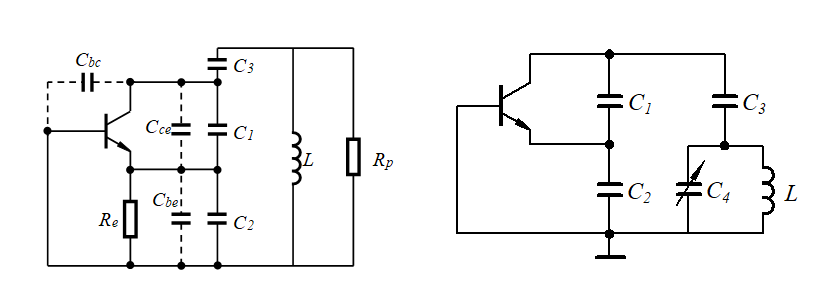
\includegraphics[scale=0.7]{image/Picture8.png}
    \caption{克拉泼、西勒电路}
\end{figure}

选取$C_3$远远小于$C_1$和$C_2$,克拉泼、西勒电路的振荡频率分别为:

\begin{equation}
    \omega_{\text{Clapp}} \approx \frac{1}{\sqrt{L C_3}}, \quad 
    \omega_{\text{Seiler}} \approx \frac{1}{\sqrt{L (C_3 + C_4)}}
\end{equation}

克拉泼电路的特点:晶体管与谐振回路是松耦合;调整$C_1$、$C_2$改变反馈系数,对谐振频率影响很小;调整$C_3$改变系统谐振频率,对反馈系数无影响;波段覆盖的范围窄;工作波段内输出波形随着频率的变化大。

西勒电路电路特点:波段覆盖率宽;工作波段内,输出幅度较平稳。

\section{晶体振荡器 \textcolor{red}{$\bigstar$}}

\subsection{晶振内部原理}

石英晶体具有正、反两种压电效应。当某一电轴受交变电场作用时,机械轴会产生机械振动,反之亦然。石英晶振的振动具有多谐性。包括基频振动和奇次谐波泛音振动。前者称为基频晶体,后者称为泛音晶体。

晶体厚度与振动频率成反比,工作频率越高,要求晶片越薄。当晶体几何尺寸和结构一定时,它本身有一个固有的机械振动频率。当外加交流电压的频率等于晶体的固有频率时,晶体片的机械振动最大,外电路中的交流电流最强,于是产生了谐振。

晶体振荡电路可分为两类:作为等效电感元件,称为并联谐振型晶体振荡器;作为串联谐振元件,称为串联谐振型晶体振荡器。

\subsection{并联型晶体振荡器}

把晶体置于反馈网络的振荡回路之中,作为一个感性元件,并与其他回路元件一起按照三端电路的基本准则组成三端振荡器。

并联谐振型晶体振荡器的两种基本形式:皮尔斯振荡电路 (c-b 型)、密勒振荡电路 (b-e 型)。

\begin{figure}[htbp]
    \centering
    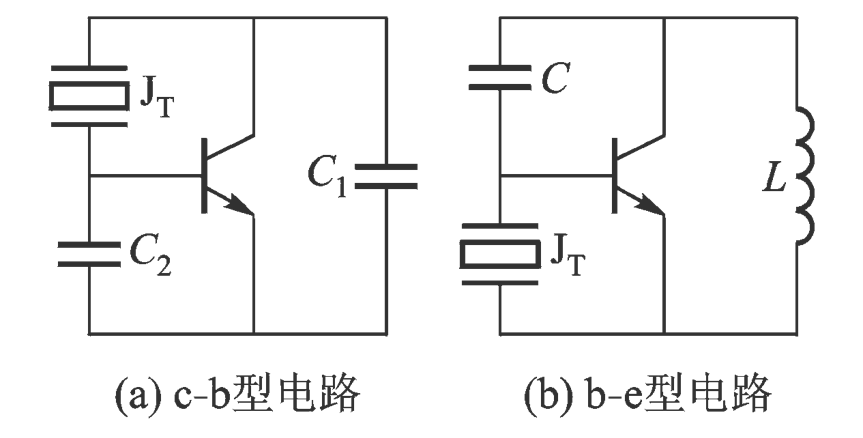
\includegraphics[scale=0.5]{image/Picture9.png}
    \caption{皮尔斯、密勒振荡电路}
\end{figure}

串联型晶体振荡器工作在 $f_q$ 与 $f_p$ 之间的一个频率点,密勒振荡电路稳定性不如皮尔斯振荡电路。

\subsection{串联型晶体振荡器}

\begin{figure}[htbp]
    \centering
    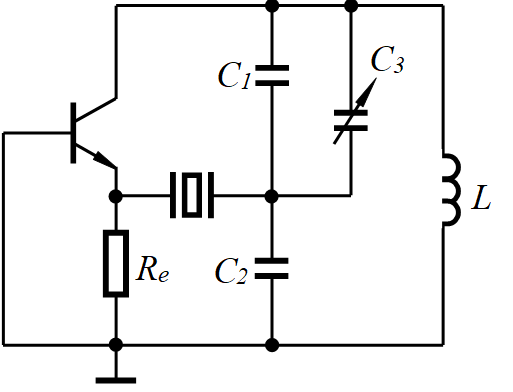
\includegraphics[scale=0.5]{image/Picture10.png}
    \caption{串联谐振型正弦波晶体振荡器电路}
\end{figure}

串联型晶体振荡器工作在 $f_{\text{osc}} = f_q$。


